\documentclass[12pt]{article}
\renewcommand{\baselinestretch}{1.5}
\usepackage[OT4]{fontenc}
\newtheorem{define}{Definition}
\usepackage{amsmath}
\usepackage{graphicx}
\usepackage{enumitem}
\usepackage{float}

\oddsidemargin=0.15in
\evensidemargin=0.15in
\topmargin=-.5in
\textheight=9in
\textwidth=6.25in

\setlength{\oddsidemargin}{.25in}
\setlength{\evensidemargin}{.25in}
\setlength{\textwidth}{6in}
\setlength{\topmargin}{-0.4in}
\setlength{\textheight}{8.5in}

\newcommand{\handout}[5]{
	\noindent
	\begin{center}
		\framebox{
			\vbox{
				\hbox to 5.78in { {\bf #1}
					\hfill #2 }
				\vspace{4mm}
				\hbox to 5.78in { {\Large \hfill #5  \hfill} }
				\vspace{2mm}
				\hbox to 5.78in { {\it #3 \hfill #4} }
			}
		}
	\end{center}
	\vspace*{4mm}
}

\newcommand{\header}[3]{\handout{NUS CS-3235: Computer Security}{\today}{Lecturer: Reza Shokri}{Student: #2\quad#3}{#1}}

%======================================
%======================================
%======================================

\begin{document}

% Indicate your name and your student number here (e.g., A01xxx)
\header{Assignment 2 Report}{Pedro Teixeira}{A0208300Y}

\section*{Notes}

\begin{itemize}
    \item Python scripts were used to generate the payloads required to perform the attacks.
    \item An effort was mad to document well the source code used to build the exploits and so it may help clarify anything omitted in this document for the sake of brevity.
    \item Each exercise's folder includes a script (\texttt{exploit.sh}) that automates the sequence of commands needed to perform the attack, and verifies that ASLR is turned off.
    \item For instructions to manually run the attacks, please refer to the README file included.
    \item In exercises 1 and 2, the buffer and global variable addresses are determined at the time the payload is built by the Python scripts, which execute the programs capturing the standard output and extracting the addresses. 
    \item All exploits were built and executed inside the VM provided for tutorial 2.
    \item The exploits in exercises 1 and 2 work well outside \texttt{gdb}. However, the exploit for exercise 3 can only be performed inside \texttt{gdb}.
\end{itemize}

%======================================
\newpage
\section{Buffer Overflow}

% Your report should include screenshots wherever you feel it is needed for better explanations similar to the tutorial notes. 

% When you use addresses in your payloads explain how you found them.

To cause a buffer overflow, all we need to ensure is that the same number of bytes is read from both the \texttt{exploit1} and the \texttt{exploit2} files, so they must have the same length to prevent the execution being stopped earlier.

We observe that the way the two initial buffers (\texttt{buf1} and \texttt{buf2}) are copied into the main buffer (\texttt{buf}) is that the bytes are interleaved, starting with a byte from \texttt{buf1}. Therefore, to write our payload to the files, we created a Python function that performs the inerse operation (given a string of bytes, splits it into two such that the buffer copying operation reconstructs the initial string).

We must also note that due to lines 19 and 20, the $64^{th}$ byte in each of the initial buffers gets overwritten with a NULL byte (0x0). Therefore, a limitation on the distance between the return address and the start of the main buffer is imposed on our traditional shellcode injection. 

Since the start of the main buffer is printed by the program, we choose to place the shellcode at that address, for simplicity.

By running the program inside \texttt{gdb} and pausing it  right after the local variables in the \texttt{bof} function variables are initialized, we observe that the return address is on the stack at address \texttt{0x7fffffffddb8}, 104 bytes away from the initial buffer address:

\begin{center}
    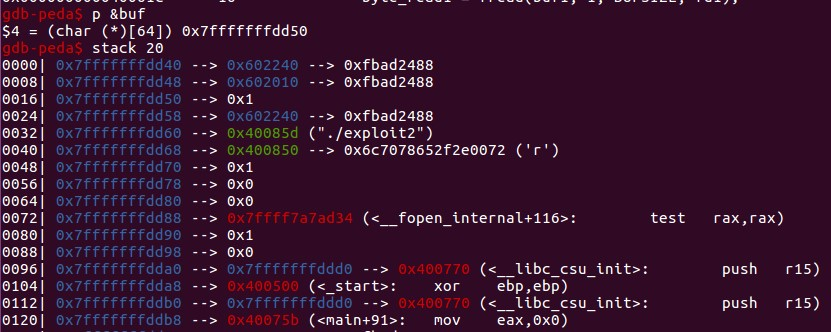
\includegraphics[scale=0.75]{ex1-ret-addr-buf.jpg}
\end{center}
 
Therefore to overflow the stack up to and including the return address we need $104 + 8 = 112$ bytes in our payload, which fits within the limitation earlier identified.

To preserve the behaviour of the copying loop and not risk it iterating forever, we must preserve the values of \texttt{byte\_read1} and \texttt{byte\_read2} and to make sure the copying is done in correct order we must also preserve \texttt{idx}.

We know that \texttt{byte\_read1} and \texttt{byte\_read2} will both take the value 56, because for a payload of 112 bytes, that is the length of each file. To determine where to put those values we can once again use \texttt{gdb}:
\begin{center}
    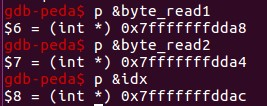
\includegraphics{ex1-var-locations.jpg}
\end{center}

The value we want to replace in \texttt{idx} is not as trivial to calculate, but basically we need to know the loop iteration in which the variable is overwritten. Since each loop iteration writes one byte we calculate the distance from the start of the buffer to the \texttt{idx} variable: \texttt{07fffffffddac - 0x7fffffffdd50 = 0x5c (92)}. Therefore we must write the value 92 on \texttt{idx}.

The final structure of our payload is as follows, totalling 112 bytes:
\begin{itemize}
    \itemsep0em 
    \item 27 bytes of shellcode
    \item 57 bytes of dummy data
    \item 4 bytes expressing the value 56 to overwrite \texttt{byte\_read1}
    \item 4 bytes expressing the value 56 to overwrite \texttt{byte\_read2}
    \item 4 bytes expressing the value 92 to overwrite \texttt{idx}
    \item 8 more bytes of dummy data
    \item 8 bytes of the address of the beginning of the buffer which contains the shellcode
\end{itemize}

The first 57 bytes of dummy data will cover the distance between the end of our shellcode and the variables we wish to overwrite with specific data. The 8 bytes of dummy data just before the return address cover the remaining distance.


%======================================

\newpage
\section{Format String Attack}

For this attack we started by running the program to identify the address of the global variable \texttt{jackpot}, which we wish to overwrites: \texttt{0x601074}.

Then we aim to construct a string that can write to that memory location when \texttt{printf()} is called with it as argument. For this we use the \texttt{\%n} format specifier, in a similar way to what is explained in the instructions for tutorial 2.

The memory location to write to can be specified as one of the argument slots of the \texttt{printf()} call. Since the first 5 arguments are passed in registers, to pass the address on the stack we must specify argument 6 or larger. Since the address needs to be aligned to 8 byte words, and the string will already contain some other bytes before the address we can specify argument 7 and then pad until its location. 

Our payload so far is: \texttt{\%7\$nAAAA\textbackslash{}x00\textbackslash{}x00\textbackslash{}x00\textbackslash{}x00\textbackslash{}x00\textbackslash{}x74\textbackslash{}x10\textbackslash{}x60}.

Note that we has to pad the address with 0s to extend it to 8 bytes.

Since all we can write is the number of characters printed before the format specifier is reached, this will write the value 0 into \texttt{jackpot}. To achieve our goal we must build our payload with 4919 characters followed by the \texttt{\%n} format specifier. To make this possible with a buffer of only 128 bytes, we use \texttt{\%4919c}, which causes 4919 spaces to be printed as padding.

Our payload so far is: \texttt{\%4919c\%7\$nAAAA\textbackslash{}x00\textbackslash{}x00\textbackslash{}x00\textbackslash{}x00\textbackslash{}x00\textbackslash{}x74\textbackslash{}x10\textbackslash{}x60}

However, now the seventh argument is no longer the correct address, but rather the substring \texttt{\$nAAAA\textbackslash{}x00\textbackslash{}x00}. To fix this, we specify the address to be the eight argument instead and add 2 more ``A''s to align it, resulting in the final payload: \texttt{\%4919c\%8\$nAAAAAA\textbackslash{}x00\textbackslash{}x00\textbackslash{}x00\textbackslash{}x00\textbackslash{}x00\textbackslash{}x74\textbackslash{}x10\textbackslash{}x60}.

This causes the address (\texttt{0x601074}) to be the third word on the stack, which corresponds to the eight argument:

\begin{center}
    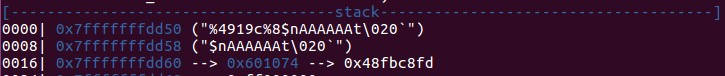
\includegraphics[scale=0.9]{ex2-stack.jpg}
\end{center}



%======================================

\newpage
\section{Return-oriented Programming}

\subsection{Creating a bufffer overflow}

The variables \texttt{i} and \texttt{fsize} are compared on line 21 to determine how many bytes are going to be read from the \texttt{exploit} file. To create a buffer overflow we just need to cause \texttt{read\_size = fsize}, which happens when \texttt{(size\_t) i < (size\_t) fsize} evaluates to false.

\texttt{i} must be at most 24 for execution to even reach this point, but it is not an unsigned variable, so it can be negative causing the type casting to \texttt{size\_t} (which is unsigned) to transform it to a very large number. If \texttt{i} is -1, the conversion will transform it to the maximum value of a long and so it must be the case that \texttt{(size\_t) i > (size\_t) fsize}.

\subsection{Determining arguments to the functions}

The \texttt{read} function needs the file descriptor returned by open. Since file descriptors 0, 1 and 2 are standard input, standard output and standard error, and the \texttt{exploit} file should already be closed at the time we call \texttt{open}, the file descriptor returned must always be 3, as they are allocated in sequence.

The buffer for the file data can be any writable memory location so we opted for a segment in \texttt{libc} that spans addresses \texttt{0x00007ffff7dd1000} to \texttt{0x00007ffff7dd7000}  which is 24576 bytes long, and was identified using the command \texttt{vmmap} in \texttt{gdb}.

The filename can be stored at the beginning of the buffer \texttt{buf}, which can be identified in \texttt{gdb}. This will vary even though ASLR is supposed to be off and so the script that generates this part of the payload always asks the user to input the value. We considered the possibility of using an environment variable, but in that case the address would also change in each new terminal session. 

\subsection{Passing arguments to the functions}

According to the observations above, we would like our gadgets to set up the following sequence of function calls:
\begin{enumerate}
    \itemsep0em
    \item \texttt{open(filename, 0)}
    \item \texttt{read(3, 0x00007ffff7dd1000, 24576)}
    \item \texttt{write(1, 0x00007ffff7dd1000, 24576)}
\end{enumerate}

For this, we will need to set two or three arguments per call. Those arguments must go into registers \texttt{rdi}, \texttt{rsi}, \texttt{rdx} in this order.

To be able to populate the registers with the values we intended, the following gadgets were identified, using the \texttt{asmsearch} command on the code and \texttt{libc} sections of memory:
\begin{itemize}
    \itemsep0em
    \item \texttt{0x00000000004008c3 : (5fc3)	pop    rdi;	ret}
    \item \texttt{0x00007ffff7a2d2e8 : (5ec3)	pop    rsi;	ret}
    \item \texttt{0x00007ffff7a0eb92 : (5ac3)	pop    rdx;	ret}
\end{itemize}

To find the addresses of the needed functions we used the \texttt{p <funcname>} in \texttt{gdb}:
\begin{itemize}
    \itemsep0em
    \item \texttt{open: 0x7ffff7b04030}
    \item \texttt{read: 0x7ffff7b04250}
    \item \texttt{write:  0x7ffff7b042b0}
\end{itemize}


\subsection{Locating the return address}

By inspecting the stack inside \texttt{gdb} we noted that the return address is 56 bytes after the beginning of the buffer we are overflowing. This means that our choice to write the filename on it will limit us to filenames of up to 55 characters long (+1 byte for null termination), but we consider this to be a reasonable limitation for this exercise. Bytes not used will be populated with ``A''s.


\subsection{Building the payload}

To execute our attack we overwrite the return address with the address of the first gadget we wish to execute. For the gadgets that pop values from the stack, we include the value to be popped right ``below'' (higher address as stack is descending) the gadget's address. Chaining all our gadgets together we end up with the following state in the stack just before the \texttt{rop} function returns (the \texttt{exit} function was added at the end for ``graceful'' termination): 

\begin{center}
    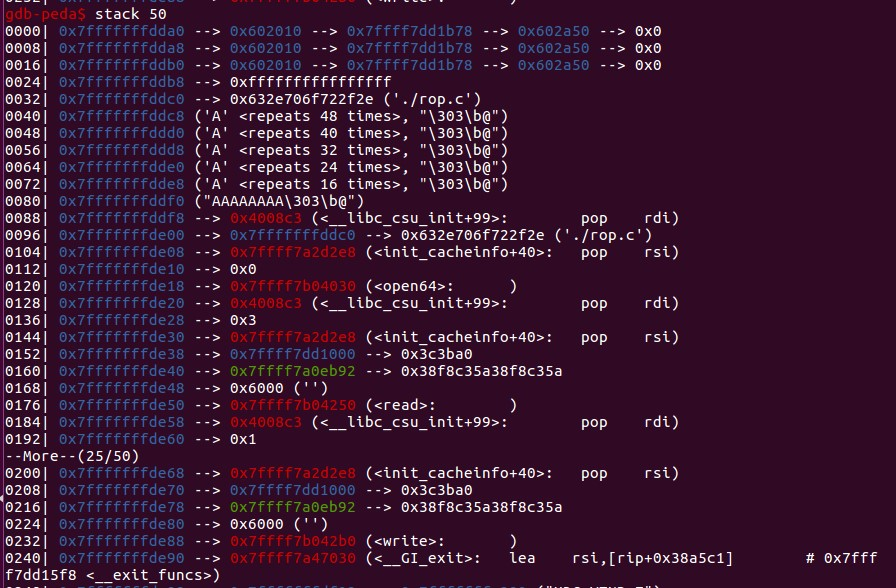
\includegraphics[scale=0.8]{ex3-stack.jpg}
\end{center}

\subsection{File length limitation}

This exploit can only print complete files if their size is up to 24576 bytes due to the size of the buffer chosen. For larger files, one could use the buffer iteratively and print one chunk of up to 24576 bytes at a time. For the purpose of this exercise we considered this a reasonable limitation and did not attempt to implement such a workaround.



\end{document}
